\documentclass[a4j,dvipdfmx]{article}
%Format   -----------------------
\usepackage[utf8]{inputenc}
\usepackage{enumitem}
\usepackage[margin=30mm]{geometry}
\usepackage{comment}
%Format   -----------------------

%Circuit ------------------------
\usepackage{amsmath,amssymb}
\usepackage[dvipdfmx]{graphicx}
\usepackage[dvipdfmx]{hyperref}
\usepackage{siunitx}
\usepackage{float}
\usepackage{tikz}
\usepackage{circuitikz}
%Circuit ------------------------

%Title   ------------------------
\title{実験レポートP3}
\author{東京大学工学部電気電子工学科 03210517\\ 藤田誠之 }
\date{April 6, 2021}
%Title   ------------------------

\begin{document}

\maketitle
\section{実験方法}

\begin{enumerate}[label={(\arabic*)}]
\item LTSpiceのインストールし、使い方を習熟する
\item Butterworth特性とChebyshev特性を持つように図1におけるL1, L2の値を決定する
\item 周波数変換及びインピーダンススケーリングを行い低域通過フィルタを設計し、回路シミュレーションで振幅特性、位相特性、ステップ応答の伝達特性を調べる
\item 規格化低域通過フィルタを基準として広域通過フィルタを設計し伝達特性をシミュレーションする
\item 規格化低域通過フィルタを基準として中心周波数および帯域幅通過フィルタを設計し伝達特性をシミュレーションする
\end{enumerate}

\iffalse
\section{実験結果}
\begin{enumerate}[label={(\arabic*)}]
\item インストールをした.
\item す
\end{enumerate}
\fi

\section{考察・検討}
\begin{enumerate}[label={(\arabic*)}]
\item Butterworth特性とChebyshev特性のLPFの周波数特性を比較せよ\\~\\

\begin{figure}[H]
    \begin{center}
     	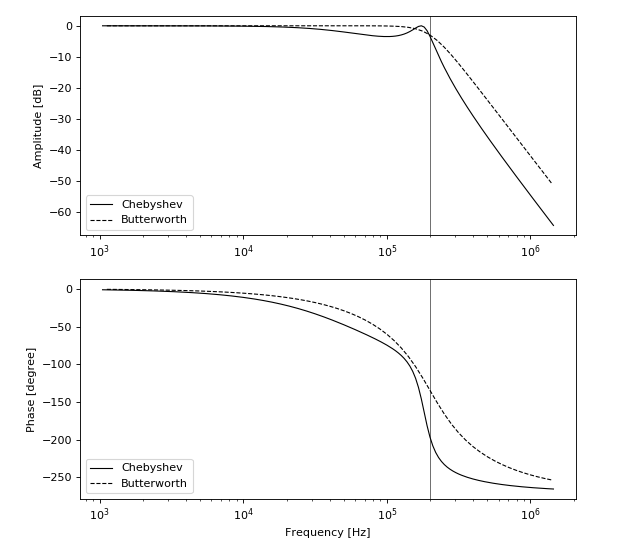
\includegraphics[width=8cm]{LPF_BC_f.png}
        \caption{LPF Frequency Response (Butterworth \& Chebyshev)}
    \end{center}
\end{figure}

\begin{figure}[H]
    \begin{center}
     	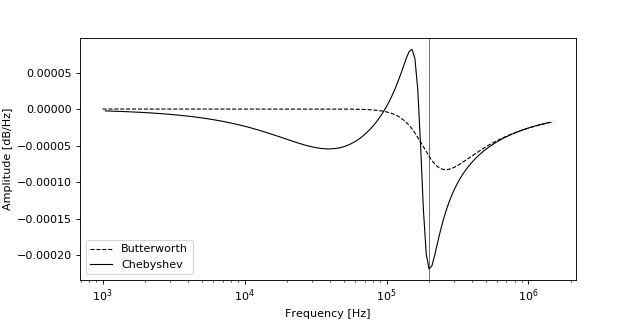
\includegraphics[width=10cm]{BC_f_amp_differential.png}
        \caption{LPF Frequency Response Differential(Butterworth \& Chebyshev)}
    \end{center}
\end{figure}

\begin{figure}[H]
    \begin{center}
     	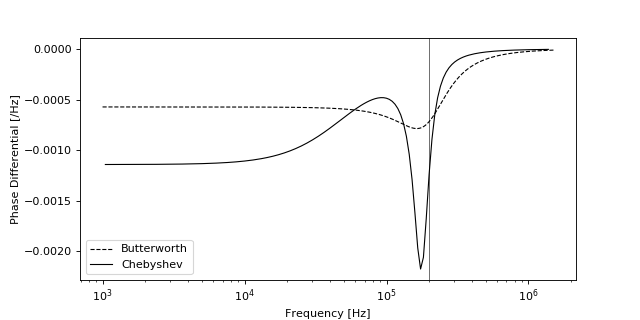
\includegraphics[width=10cm]{BC_f_phase_differential.png}
        \caption{LPF Frequency Response Differential(Butterworth \& Chebyshev)}
    \end{center}
\end{figure}

実験結果は上図のようになった。カットオフ周波数は200kHzとして設計をした。Figure 2はFigure 1の振幅のデータを微分したものである。Figure 2を見ると、Butterworthフィルタは0.0を超えていないことがわかる。つまり、Butterworthフィルタでは周波数が上がるにつれ単調減少しているということがわかる。一方、Chebyshevフィルタでは一度減少した後、200kより手前で増加に転じ、0に近づいたあと再び減少している。両者とも、200kを超えてからは、両対数グラフにおいて直線に近似できるが、Butterworthフィルタの方が振幅の減少が遅いこともわかる。さらに、Figure 2を見ると、200kHzにおいて振幅の微分が減少していることがわかるが、これはFigure 1の振幅のグラフにおいて通過域から遮断域へ移るときの「角の強さ」を表していると考えることができる。ButterworthフィルタとChebyshevフィルタを比較すると、Chebyshevフィルタのほうが急激に微分が減少している、つまり切り替わりがより急であるということである。また、Figure 3は位相特性を微分したものであるが、200k付近で位相が急激に変化していることが分かる。この変化はChebyshevフィルタの方が強いということも分かる。\\~\\

また、以下のようなグラフも作成した。
\begin{figure}[H]
    \begin{center}
     	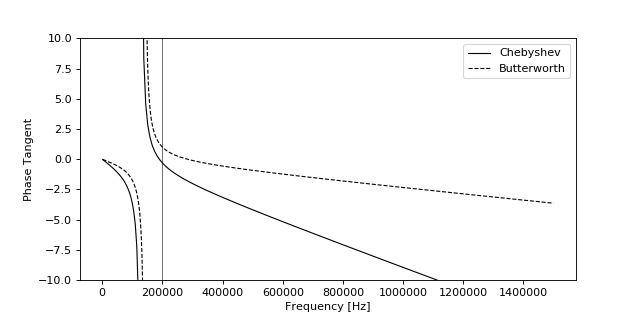
\includegraphics[width=10cm]{BC_f_phase_tangent.png}
        \caption{LPF Frequency Response Differential(Butterworth \& Chebyshev)}
    \end{center}
\end{figure}
これは、位相のtangentの値をプロットしたものである。周波数が200kHzを超えたところで直線となっている。何かしら意味があるのかと思うが、レポートの提出期限までにはわからなかった。


\item 3次のLPFは、高周波における伝達関数が$1/s^3$で近似できるはずである。振幅特性、位相特性からこのことを確認せよ。
\\~\\ 今回のLPFの回路図は以下のようになる。\\
\begin{figure}[H]
  \begin{center}
    \begin{circuitikz}[american currents]
     \ctikzset{american inductors}
	  \draw (0,0)
      to[sV=$V_s$] (0,2)
      to[L=$L_1$] (3,2)
      to[C=$C$] (3,0)
      to[short] (0,0);
      \draw (3,2)
      to[L=$L_2$] (6,2)
      to[european resistor=$1\Omega$] (6,0)
      to[short] (3,0);
    \end{circuitikz}
    \caption{3次規格化0-R型LPF}
  \end{center}
\end{figure}

伝達関数を計算すると以下のようになる。

$$
\frac{V_2}{V_1} = \frac{1}{s^3L_1L_2C+s^2CL_1+s(L_1+L_2)+1}(=F(s))
$$


Butterworthについては$L_1 = 1.5, L_2 = 0.5, C = 1.333$、Chebyshevについては$L_1 = 2.158, L_2 = 1.123, C = 1.833$と求まる。また、伝達関数は、Butterworthについては$F(s)=\frac{1}{s^3+2s^2+2s+1}$、Chebyshevについては$F(s)=\frac{1}{4.44s^3+2.424s^2+3.991s+1}$で表されるが、カットオフ周波数以上でのグラフの傾きを算出した。200kHz以上のデータを使い、周波数の値の底10の対数をとった値を独立変数、振幅の値(dB)を従属変数とし、最小2乗法を用いて算出した。結果は、ButterworthフィルタとChebyshevフィルタでそれぞれ以下のようになった。
\begin{table}[H]
    \begin{center}
        \begin{tabular}{|l|c|} \hline
            Butterworth & -2.9165 \\ \hline
            Chebyshev & -3.3836 \\ \hline
        \end{tabular}
        \caption{LPF Frequency Response Slope}
    \end{center}
\end{table}

両対数グラフでの傾きは、関数の指数を表すため、3次のLPFにおいて高周波数では伝達関数が$1/s^3$と近似するとButterworthフィルタでは2.783\%,Chebyshevフィルタでは12.7\%の誤差率で近似できているということが分かる。
Butterworthフィルタの伝達関数を$s=\infty$でテイラー展開すると、
$$
\frac{1}{s^3+2s^2+2s+1} = \frac{1}{x^3} + O(\frac{1}{x^4})
$$
となるため、sが十分大きければ伝達関数$\frac{1}{s^3}$で近似できると考えることができる。Chebyshevフィルタについても同じである。
\item ButterWorth特性とChebyshev特性のLPFのステップ応答を比較せよ。周波数特性の違いはステップ応答のどこに現れているか論ぜよ。

\begin{figure}[H]
    \begin{center}
     	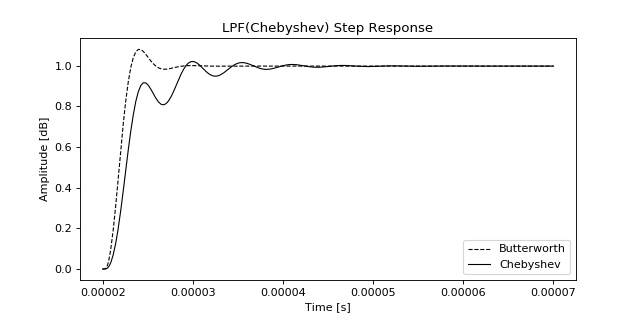
\includegraphics[width=10cm]{LPF_BC_s.png}
        \caption{LPF Step Response (Butterworth \& Chebyshev)}
    \end{center}
\end{figure}
LPFに方形波を入力した場合の出力は振動する。上のFigure 6がButterworthフィルタとChebyshevフィルタのステップ応答である。グラフを比較すると、Chebyshevフィルタの方がButterworthフィルタに比べて振動が多いことが分かる。Butterworthフィルタはオーバーシュートした後に比較的に速やかに収束している。一方、Chebyshevフィルタは振動を複数回繰り返してから収束しており、Butterworthフィルタより収束が遅いように見受けられる。

\item HPFの設計\\
Butterworth, Chebyshevを用いてHPFを設計した。$\mbox{H}_{\mbox{cutoff}}$が200kHzとなるように設計し、LPFと同様に周波数応答とステップ応答を記録した。回路図と結果はそれぞれ以下のようになった。

\begin{figure}[H]
  \begin{center}
    \begin{circuitikz}[american currents]
     \ctikzset{american inductors}
	  \draw (0,0)
      to[sV=$V_s$] (0,2)
      to[C=$C_1$] (3,2)
      to[L=$L$] (3,0)
      to[short] (0,0);
      \draw (3,2)
      to[C=$C_2$] (6,2)
      to[european resistor=$1\Omega$] (6,0)
      to[short] (3,0);
    \end{circuitikz}
    \caption{3次規格化0-R型HPF}
  \end{center}
\end{figure}

\begin{figure}[H]
    \begin{center}
     	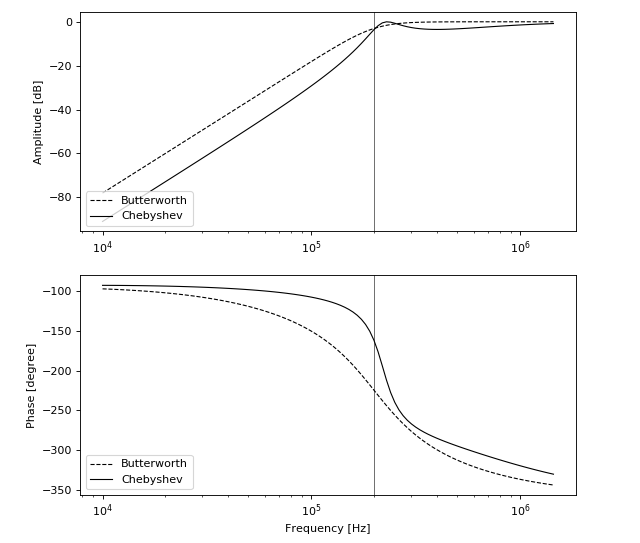
\includegraphics[width=10cm]{HPF_BC_f.png}
        \caption{HPF Frequency Response (Butterworth \& Chebyshev)}
    \end{center}
\end{figure}

\begin{figure}[H]
    \begin{center}
     	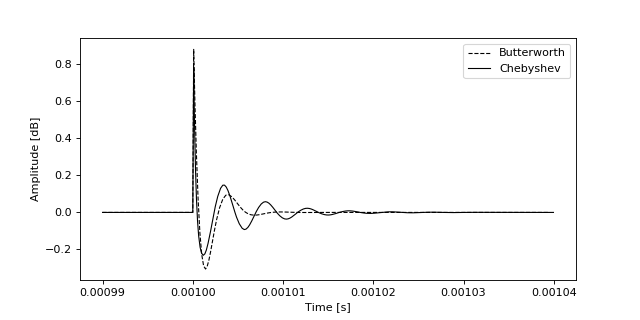
\includegraphics[width=10cm]{HPF_BC_s.png}
        \caption{HPF Step Response (Butterworth \& Chebyshev)}
    \end{center}
\end{figure}

200kHz未満の傾きを調べると、以下のようになった。

\begin{table}[H]
    \begin{center}
        \begin{tabular}{|l|c|} \hline
            Butterworth & 2.9558 \\ \hline
            Chebyshev & 3.2232 \\ \hline
        \end{tabular}
        \caption{HPF Frequency Response Slope}
    \end{center}
\end{table}

このことから、伝達関数がどちらも低周波数域では$s^3$で近似できるということが分かる。実際、伝達関数を計算すると
$$
F = 
\left(
\begin{array}{cc}
	1 & \frac{1}{sC_1}\\
	0 & 1\\
\end{array} \right)
\left( \begin{array}{cc}
	1 & 0\\
	\frac{1}{sL} & 1\\
\end{array} \right)
\left( \begin{array}{cc}
	1 & \frac{1}{sC_2}\\
	0 & 1\\
\end{array} \right)
=
\left( \begin{array}{cc}
	1+\frac{1}{s^2LC_1} & \frac{1}{sC_2}\left(1+\frac{1}{s^2LC_1}\right) +\frac{1}{sC_1}\\
	\frac{1}{sL} & \frac{1}{s^2LC_2}+1\\
\end{array} \right)
$$
$$
F(s) = \frac{s^3LC_1C_2}{s^3LC_1C_2+s^2L(C_1+C_2)+sC_2+1}
$$
これを$s=0$でテイラー展開すると
$$
F(s)=As^3+O(s^4) \mbox{ (Aは定数)}
$$
となるので、sが十分小さければ伝達関数は$s^3$で近似できることが分かる。

\item BPFの設計\\
Butterworth, Chebyshevを用いてBPFを設計した。BPFの回路図は以下のようになる。

\begin{figure}[h]
  \begin{center}
    \begin{circuitikz}[american currents]
     \ctikzset{american inductors}
	  \draw (0,0)
      to[sV=$V_s$] (0,4)
      to[L = $L_1$] (2,4)
      to[C=$C_1$] (4,4)
      to[short] (4,3)
      to[short] (3,3)
      to[L = $L_3$] (3,1)
      to[short] (4,1)
      to[short] (4,0)
      to[short] (0,0);
      \draw (4,3)
      to[short] (5,3)
      to[C=$C_3$] (5,1)
      to[short] (4,1);
      \draw (4,4)
      to[L = $L_2$] (6,4)
      to[C=$C_2$] (8,4)
      to[european resistor=$1\Omega$] (8,0)
      to[short] (4,0);
    \end{circuitikz}
    \caption{3次規格化0-R型HPFD}
  \end{center}
\end{figure}

周波数応答とステップ応答は以下の図のようになった。

\begin{figure}[H]
    \begin{center}
     	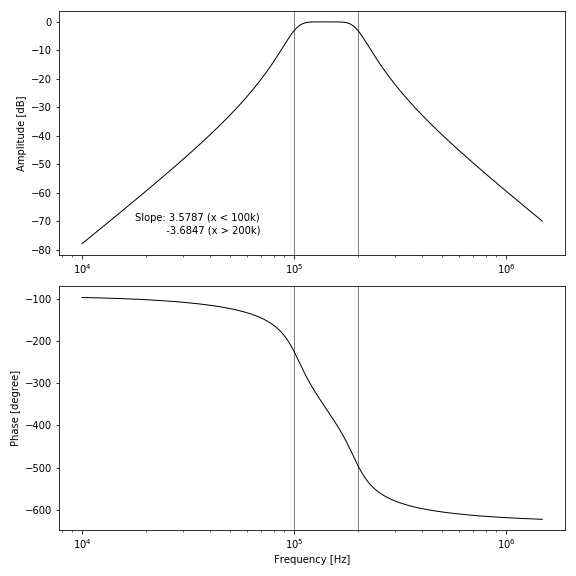
\includegraphics[width=7cm]{BPF_B_f.png}
        \caption{BPF Response (Butterworth)}
    \end{center}
\end{figure}

\begin{figure}[H]
    \begin{center}
     	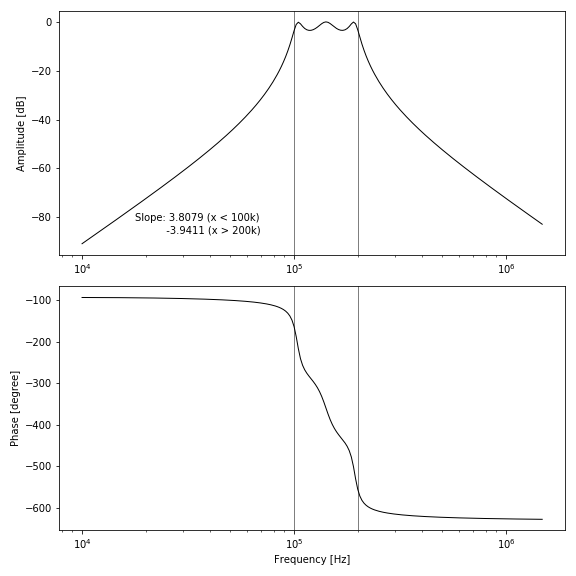
\includegraphics[width=7cm]{BPF_C_f.png}
        \caption{BPF Response (Chebyshev)}
    \end{center}
\end{figure}

\begin{figure}[H]
    \begin{center}
     	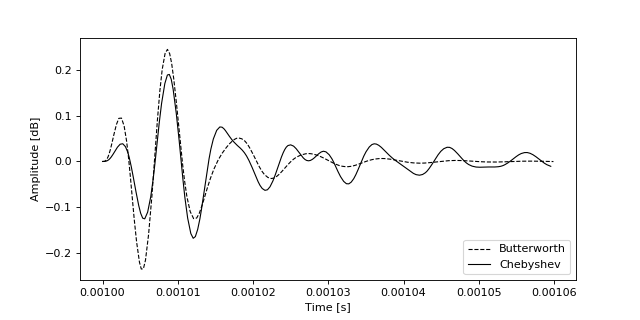
\includegraphics[width=10cm]{BPF_BC_s.png}
        \caption{BPF Response (Chebyshev)}
    \end{center}
\end{figure}

\begin{table}[H]
    \begin{center}
        \begin{tabular}{|l|l|c|} \hline
        	& $\leq 100kHz$ & $\geq200kHz$\\ \hline
            Butterworth & 3.5787 & -3.6847\\ \hline
            Chebyshev & 3.8079 & -3.9411\\ \hline
        \end{tabular}
        \caption{LPF Frequency Response Slope}
    \end{center}
\end{table}

振動や応答については、LPFとHPFと似たような動き、つまりButterworthフィルタに比べてChebyshevフィルタは振動が多く、また傾きが大きいということが分かる。また、ステップ応答に関しては、Butterworthフィルタのほうがオーバーシュートが大きかった。伝達関数を計算すると、適当な係数を用いて$F=a_1s^3+a_2s^2+a_3s+a_4+a_5s^{-1}+a_6s^{-2}+a_7s^{-3}$と表すことができる。つまり、低周波数領域では$F(s) = s^3$と近似でき、高周波数領域では$F(s) = s^{-3}$と近似できることが分かる。実際、傾きを調べるとおおよそこの近似が成り立っていることが分かる。

\item BEFの設計\\
ButterworthとChebyshevを用いてBEFフィルタを設計した。周波数応答、ステップ応答は以下の通りになった。

\begin{figure}[H]
    \begin{center}
     	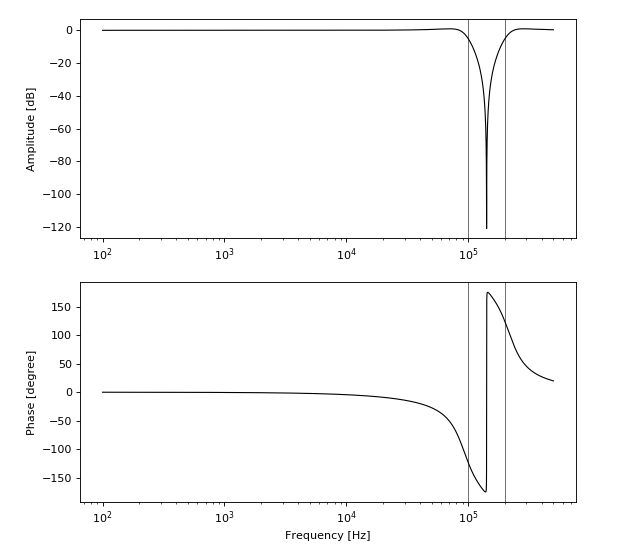
\includegraphics[width=10cm]{BEF_B_f.png}
        \caption{BPF Frequency Response (Butterworth)}
    \end{center}
\end{figure}

\begin{figure}[H]
    \begin{center}
     	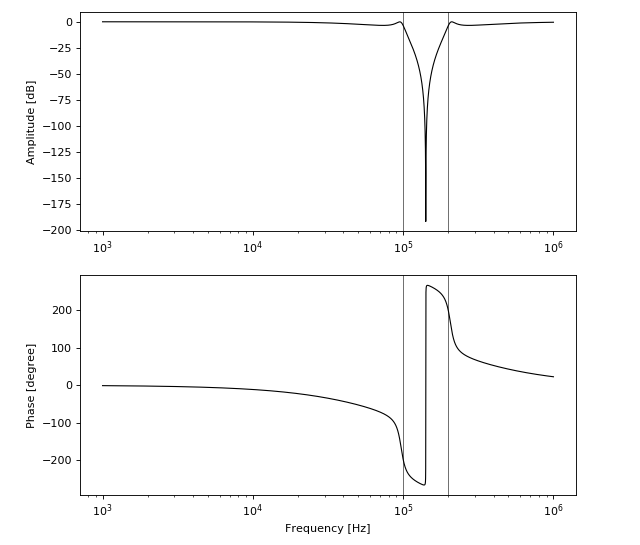
\includegraphics[width=10cm]{BEF_C_f.png}
        \caption{BPF Frequency Response (Chebyshev)}
    \end{center}
\end{figure}


周波数応答では、100kHzから200kHzまでのバンドの信号が弱まっていることが分かる。また、中間の150kHz付近で位相が大きく(約360度)変化していることも分かる。ステップ応答ではButterworthフィルタがオーバーシュートしていることが分かる。
\section{参考文献}
『計測とフィルタ(その2:フィルタの周波数特性と波形応答)』\url{<https://www.orixrentec.jp/helpful_info/detail.html?id=43>} 2020年4月14日アクセス
\end{enumerate}
\end{document}